
\newpage % Rozdziały zaczynamy od nowej strony.
\section{Podjęta problematyka}
Zjawisko intencjonalnego publikowania nieprawdziwych informacji dostało nazwę fake news. 
Ten neologizm został również zaadoptowany w\,języku polskim. Słownik języka polskiego PWN w\,dziale ciekawostki definiuje zwrot fake news jako „nieprawdziwe, fałszywe wiadomości, najczęściej rozpowszechniane przez tabloidy w\,celu wywołania sensacji, bądź zniesławienia kogoś (najczęściej polityka)”. Według językoznawcy nie jest to w\,języku polskim już tylko słowo slangowe, jako że wygrało w\,plebiscycie słowników Collinsa w\,roku 2017\footnote{\url{https://sjp.pwn.pl/ciekawostki/haslo/fake-news;6368870.html}}.  Inaczej możemy to zjawisko nazywać dezinformacją, które jest definiowana jako „fałszywa, rzekoma informacja, zamierzone wprowadzenie w\,błąd” \footnote{\url{https://sjp.pl/dezinformacja}}. 
Może ono objawiać się pod różnymi formami, najbardziej kojarzą się z\,ich pierwotną formą jaką są artykuły w\,mediach szerzące nieprawdę. Mimo że ten problem występuje tak długo jak istnieją media obecnie jednak jego wpływ jest dużo większy. 

\subsection{Problematyka nierzetelnych informacji}
Szerzenie się nieprawdziwych, nierzetelnych informacji w\,mediach, z\,których pobieramy wiedzę o świecie nie może być ignorowane. Wielkość tego zjawiska już teraz stwarza dużo problemów i \,ciągle się powiększa. Coraz więcej osób pobiera najświeższe informacje o wydarzeniach z\,internetu. Informacje można te podzielić ze względu na źródło z\,jakiego pochodzą. Mogą być one bowiem publikowane przez tradycyjne media znane z\,formy papierowej lub telewizyjnej posiadające własną stronę internetową. Ale internet daje również duże możliwości publikowania własnych treści wszystkim użytkownikom, dzieje się to głównie poprzez blogi i\,portale społecznościowe.  \par
Nierzetelne informacje w\,Internecie są poważnym problemem. 68\% Europejczyków natrafia na informacje, które zakłamują rzeczywistość przynajmniej raz w\,tygodniu a\,połowa z\,nich nawet codziennie \cite{Eurobarometer4642018}. Na szczęście 71\% z\,nich twierdzi, że jest raczej pewnych w\,swoich umiejętnościach wykrycia czy czytana przez nich informacja o wydarzeniach jest prawdziwa czy też nie. Mimo to nierzetelne informacje występują w\,mediach społecznościowych a\,użytkownicy często wchodzą z\,nimi w\,interakcje poprzez udostępnianie ich dalej.
\par Mimo tego, że więcej użytkowników Internetu nadal bardziej ufa źródłom związanym z\,tradycyjnymi mediami niż informacjom generowanym przez użytkowników \cite{rieh2014credibility} to według badań z\,2018 roku 68 procent ankietowanych amerykanów zadeklarowało, że zdarza im się czytać informacje za pomocą portali społecznościowych \cite{PewNewsUse2018}. Takie badania co roku przeprowadza Centrum Badań Pew. Według ich danych wzrost liczby osób korzystających z\,portali społecznościowych do zdobywania wiadomości o świecie w\,ostatnim roku przystopowała po czasie dużego wzrostu w\,poprzednich latach.

\subsubsection{Social media}
Widać, więc jak duże jest nadal znaczenie portali społecznościowych w\,szerzeniu informacji. Dzieje się tak z\,kilku powodów. Dla użytkowników jest to po prostu wygodne. Przeglądając główną stronę aplikacji użytkownik dostaje posty subskrybowanych przez siebie stron informacyjnych lub posty z\,którymi weszli w\,interakcje jego znajomi. Dzieje się tak w\,szczególności dla portalu Facebook, gdzie większość użytkowników spotyka posty informacyjne robiąc inne rzeczy na portalu a \,nie szukając ich specjalnie \cite{PewNewsUse2016}. Takie pobieranie informacji nie wymaga od użytkownika większego wysiłku a\,daje duże możliwości. Są one świetnym źródłem informacji o najświeższych wydarzeniach jak również relacji naocznych świadków wydarzeń lub wypowiedzi osób bezpośrednio z\,nimi związanych. Użytkownik dodatkowo może wchodzić w\,interakcję z\,innymi odbiorcami. W\,łatwy sposób może komentować i \,uczestniczyć w\,dyskusji na wybrane przez siebie tematy. Popularność portali społecznościowych wykorzystują więc wszystkie instytucje, które chcą przekazać informację lub swoją opinię. Krótkie notki publikowane na takich portalach mogą powstawać szybko i \,małym kosztem w\,porównaniu do pełnowymiarowego artykułu. 
\par Niestety wszystkie wymienione wyżej czynniki tworzą doskonałe podłoże do szerzenia dezinformacji. Każdy może napisać cokolwiek chce. Świeże posty bardzo ciężko jest zweryfikować pod względem prawdziwości a \,mogą szybko zostać rozniesione między użytkownikami serwisu. Głównym problemem w\,rozprzestrzenianiu dezinformacji lub treści o tematyce konspiracyjnej mogą być sami użytkownicy. Badania wykazały, że posty publikowane przez strony zakwalifikowane jako konspiracyjne otrzymują więcej ‘polubień’ oraz udostępnień przez użytkowników niż posty publikowane przez portale naukowe \cite{bessi2015science}. 

\subsection{Powody popularności Fake News}
Należy się zastanowić, dlaczego w\,ogóle część użytkowników preferuje przyjmowanie wiadomości, które nie są prawdziwe. Można by założyć, że większość społeczeństwa nie akceptuje bycia okłamywanym. Dlaczego więc jakaś grupa toleruje otaczające go fałszywe informacje.  Problem ten nie występuje tylko w\,oparciu o\,informacje przekazywane przez media społecznościowe, ale również media tradycyjne takie jak czasopisma, radio i\,telewizja. 
\par Powody, dla których poddajemy się przyjmowaniu fałszywych informacji możemy podzielić na dwa rodzaje: psychologiczne i \,społeczne \cite{shu2017fake}. Te pierwsze są w\,szczególności wykorzystywane przez media tradycyjne, które samemu wybieramy, natomiast społeczne są wyjątkowo nasilone, jeśli mamy możliwość lub musimy wyrazić głośno swoją opinię.

\subsubsection{Czynniki psychologiczne}
Psychologiczne powody sięgania po określone treści mogą być spowodowane zjawiskiem nazwanym naiwnym realizmem. Polega ono na tym, że człowiek sądzi, że to co on wie lub w\,co wierzy jest jedyną prawdą, a\,jeśli się koś z\,nim nie zgadza to musi być niedoinformowany lub nieracjonalny. Jest to powiązane z\,efektem potwierdzenia. Jest to zjawisko w\,psychologii, gdzie człowiek zawsze będzie wybierał informacje, które potwierdzają jego wcześniej utarte przekonania. Prowadzi to również do selektywnego wybierania dowodów oraz interpretowania ich na korzyść swoich przekonań.  Występuje to w\,szczególności przy tematach, którym towarzyszą skrajne opinie i \,duże emocje. Przy tym często taka opinia jest oparta na pierwszych informacjach, które przyswoił. Dlatego ludzie czasem sięgają po konkretne informacje nie zważając na ich prawdziwość.  Dodatkowo bardzo trudno jest zmienić zdanie takiej osoby. Przedstawianie im treści, która naprostowuje nierzetelne informacje często nie daje żadnych efektów lub wręcz pogłębia ich wcześniejszą opinię. 

\subsubsection{Czynniki społeczne}
Człowiek jest istotą społeczną, można więc powiedzieć, że jedną z\,jego głównych potrzeb jest przynależność do grupy i \,bycie akceptowanym przez innych. Jest to nawet zaznaczone w\,modelu hierarchii potrzeb Maslowa. Ta podświadoma potrzeba może objawiać się w\,taki sposób, że osobnik będzie wyrażał opinię, która jest popularna w\,jego otoczeniu. Oznacza to zarówno, że będzie preferował odbieranie informacji, które nawiązują do przekonań jego grupy. Może się to utrzymać również w\,sytuacji, kiedy te informacje są spaczone lub stronnicze. Mimo to dla osobnika będzie to wybór społecznie bezpieczny.

\subsection{Efekt komory pogłosowej}
Media społecznościowe dają jeszcze większe możliwości przyjmowania informacji, wyrażania głośno swojej aprobaty i \,emocji jakie wywołują oraz dyskusji na ich temat z\,innymi użytkownikami. Dodatkowo można w\,łatwy sposób wybierać preferowane źródła, które publikują preferowane przez nas tematy lub opinie. Mimo wielu zalet takich jak wygoda w\,otrzymywaniu interesujących nas wiadomości i \,ciekawostek może to tworzyć efekt komory pogłosowej (ang. echo chamber effect) \cite{garimella2018political}. Charakteryzuje się on zjawiskiem, że użytkownik na portalu społecznościowym otacza się znajomymi o podobnych do siebie poglądach oraz subskrybuje kanały publikujące informacje, które uznaje za ciekawe, często takie z\,których opinią się zgadza. Dodatkowo najczęściej wykazuje aktywność poprzez dodanie reakcji do postu, udostępnienie go w\,przypadku treści z\,którymi zdecydowanie się zgadza lub budzą w\,nim duże emocje. Takie działania dają informację algorytmom portali na temat preferowanych przez użytkownika postów. Takie algorytmy stworzone są w\,celu zwiększenia ruchu na portalu co jest wykonywane między innymi przez zwiększenie satysfakcji użytkownika z\,otrzymywanych treści.  Algorytm wybiera więc posty odpowiadające stworzonym warunkom dla poszczególnego użytkownika. Takim sposobem tworzy się bańka komory pogłosowej. Użytkownik i \,osoby o podobnych opiniach będą otrzymywały pasujące dla nich treści. 
\par To zjawisko może być użyte do szerzenia dezinformacji. Pomagają temu dodatkowe czynniki wpływające na użytkownika  \cite{shu2017fake}. Pierwszą z\,nich jest wiarygodność społeczna, która polega na założeniu, że im więcej osób uznaje informację, lub całe źródło informacji za wiarygodne tym bardziej prawdopodobne, że inni również uznają ją za wiarygodne. W\,mediach społecznościowych jest to powiązane ze zjawiskiem heurystyki dostępności, które w\,tym kontekście można przedstawić przy pomocy niesławnego powiedzenia „Kłamstwo powtarzane wiele razy staje się prawdą”. Oznacza to, że jeśli usłyszymy pewną informację wystarczająco dużo razy, tym bardziej prawdopodobne, że uwierzymy w\,jej prawdziwość nawet gdy tak nie jest. Oba te czynniki występują w\,dużej ilości w\,mediach społecznościowych przy tworzących się bańkach komory pogłosowej i \,są bardzo podatne na rozsyłanie dezinformacji w\,taki sposób, aby użytkownicy ją akceptowali lub wręcz w\,nią uwierzyli. 

\subsection{Wpływ na rzeczywistość}
Najbardziej popularnym przykładem roznoszenia fałszywych informacji na dużą skalę jest okres przed wyborami prezydenckimi w\,Stanach Zjednoczonych w\,2016 roku. Zostało stwierdzone, że na portalu Twitter więcej udostępnień zostało wykonanych na postach zawierających fałszywe informacje niż na tych z\,prawdziwymi danymi  \cite{neudertpolarization2018}. Podobne badania przeprowadzono w Unii Europejskiej w czasie poprzedzającym wybory do europarlamentu. W przedstawionych wynikach na rysunku \ref{fig:EUMapJunkNews} wykazano, że w badanych krajach średnia liczba treści z nierzetelnych źródeł to 4\% jednak dla danych polskojęzycznych aż 20\% zebranych treści pochodziło z źródeł uznanych przez ekspertów jako nierzetelne\cite{marchal2019junk}.
\begin{figure}[!h]
	
	\centering 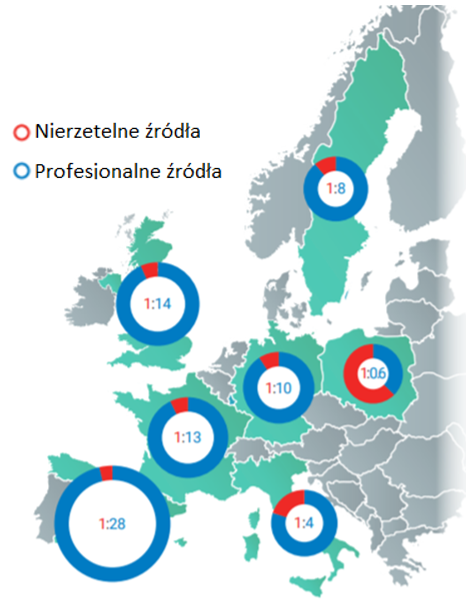
\includegraphics[width=0.5\linewidth]{img/EUMapJunkNews.PNG}
	\caption{Porównanie liczby treści ze źródeł nierzetelnych oraz profesjonalnych w wybranych państwach Unii Europejskiej. Źródło: \cite{marchal2019junk}}
	\label{fig:EUMapJunkNews}
\end{figure}
\par
Dodatkowo rozsiewanie fałszywych informacji może mieć tak tragiczne skutki jak afera Pizzagate\,\footnote{\url{https://www.nytimes.com/2016/12/05/business/media/comet-ping-pong-pizza-shooting-fake-news-consequences.html}}. Pewien człowiek uwierzywszy w\,teorię spiskową na temat mafii pedofilskiej powiązanej z\,Hillary Clinton wszedł uzbrojony do pizzerii, w\,której miał się odbywać nielegalny proceder i \,otworzył ogień. Na szczęście w\,zajściu nikt nie ucierpiał. Mimo, że przytoczony przykład jest skrajną sytuacją, pokazuje jak łatwo jest manipulować jednostkami. Największy problem pojawia się, jeśli uda się zmanipulować całą masą ludzi. 
\subsection{Podsumowanie problemu}
Fałszywe informacje są często bardzo trudne do wykrycia a\,wciąż rozwijające się algorytmy mogą być używane do szerzenia ich na ogromną skalę. Coraz częściej zaczynamy mówić o problemie wiarygodności w\,dostarczanych nam mediach. Użytkownicy korzystający z\,platform społecznościowych do czytania wiadomości też już zauważyli ten problem. Według najnowszych badań Pew 57\% użytkowników uważa takie informacje za niedokładne \cite{PewNewsUse2018}. Za główne problemy takiego zjawiska wskazują stronniczość polityczną oraz niską jakość publikowanych treści. Nie bez znaczenia jest też zachowanie innych użytkowników. 
\par Żmudne zadanie neutralizacji fałszywych informacji prowadzą już od dawna dedykowane temu portale amerykańskie. W\,polskim Internecie powstał serwis Demagog, który za cel stawia sobie sprawdzanie prawdziwości wypowiedzi polityków. Do walki z\,rozszerzającymi się fałszywymi informacjami włącza się również technologia. Powstaje coraz więcej prób zautomatyzowania wykrywania niewiarygodnych źródeł i\,artykułów mówiących nieprawdę. Automatyczne wykrywanie fake news jest to przewidywanie szans, że konkretny artykuł jest intencjonalnie fałszywy \cite{threeTypeOfFakes2015}. Niestety w\,tak szybko rozwijającym się środowisku jest to zadanie co najmniej trudne. Nie istnieją jeszcze wystarczająco dobre rozwiązania. Należy więc szukać nowych i\,dodatkowo rozszerzać je na inne języki oprócz języka angielskiego. 
